\documentclass{beamer}
\usepackage{amsmath, amssymb, amsthm}
\usepackage{graphicx}

\newcommand{\RR}{\mathbb{R}}

\title{The R\"{o}ssler System}
\author{Steven Rosendahl}
\date{}

\usetheme{Rochester}
\usecolortheme{whale}

\begin{document}

\begin{frame}
	\titlepage
\end{frame}

\begin{frame}{Introduction}
	\begin{itemize}
		\item Created by Otto R\"{o}ssler in 1976
		      \pause
		\item System constructed to display simplest possible \textit{Strange Attractor}
		      \pause
	\end{itemize}
	\begin{definition}
		An \alert{attractor} is a set of values towards which a system moves when initial conditions are \textit{near} the attractor.
		\pause
		An attractor is called \alert{strange} if it exhibits fractal behavior.
	\end{definition}
	\pause
	\begin{itemize}
		\item Strange attractors are often associated with chaotic systems.
	\end{itemize}
\end{frame}

\begin{frame}{System}
	\begin{align*}
		\dot{x} & = -y-z     \\
		\dot{y} & = x+ay     \\
		\dot{z} & = b+z(x-c)
	\end{align*}
	\pause
	\begin{itemize}
		\item $a,b,c$ are responsible for attractive behavior
		      \pause
		\item Want to analyze the effect small $a$ and $b$ have on system
		      \pause
		      \begin{itemize}
		      	\item Is the system globally stable? Locally?
		      	      \pause
		      	\item When does chaotic behavior occur?
		      \end{itemize}
	\end{itemize}
\end{frame}

\begin{frame}{First Glance}
	\begin{itemize}
		\item Finding fixed points
	    \pause
	\end{itemize}
	\begin{center}
		\scalebox{0.75}{
			\texttt{Solve[f[x, y, z] == 0 \&\& g[x, y, z] == 0 \&\& h[x, y, z] == 0, \{x, y, z\}]}
		}
	\end{center}
	\pause
	\begin{columns}[T]
		\begin{column}{0.48\textwidth}
			\[
				\begin{cases}
					x=\frac{1}{2}\left(c-\sqrt{c^{2}-4ab}\right)                     \\
					y=\frac{1}{2}\left(\frac{\sqrt{c^{2}-4ab}}{a}-\frac{c}{a}\right) \\
					z=\frac{c-\sqrt{c^{2}-4ab}}{2a}
				\end{cases}
			\]
		\end{column}
		\begin{column}{0.48\textwidth}
			\[
				\begin{cases}
					x=\frac{1}{2}\left(c+\sqrt{c^{2}-4ab}\right)                      \\
					y=\frac{1}{2}\left(-\frac{\sqrt{c^{2}-4ab}}{a}-\frac{c}{a}\right) \\
					z=\frac{c+\sqrt{c^{2}-4ab}}{2a}
				\end{cases}
			\]
		\end{column}
	\end{columns}
\end{frame}

\begin{frame}{Simplification}
    \begin{itemize}
        \item Let $a,b$ tend to zero
        \pause
        \item Cannot actually be zero (division by 0 at fixed points)
        \pause
    \end{itemize}
    \[\left\{x = 0\qquad y = 0\qquad z = 0\right\}\]
    \pause
    \[\left\{x = c\qquad y = -\frac{c}{a}\qquad z = \frac{c}{a}\right\}\]
    \pause
    \begin{itemize}
        \item Much easier to analyze stability of system
    \end{itemize}
\end{frame}

\begin{frame}{Linearization}
    \begin{itemize}
        \item Can take Jacobian of system to analyze stability
        \pause
        \item Which stabilities are hyperbolic in a 3D system?
        \pause
    \end{itemize}
    % \begin{definition}
    %     When $\lambda_{1}$, $\lambda_{2}$, and $\lambda_{3}$ are in $\RR$ and they all have the same sign, the fixed point is a \alert{node}.
    % \end{definition}
    % \pause
    % \begin{definition}
    %     When $\lambda_{1}$, $\lambda_{2}$, and $\lambda_{3}$ are in $\RR$ and at least one is positive and one is negative, the fixed point is a \alert{saddle}.
    % \end{definition}
    \begin{definition}
        When $\lambda_{1}\in\RR$ and $\lambda_{2},\lambda_{3}$ are complex conjugates \textit{and} the real part of $\lambda_{1},\lambda_{2}$, and $\lambda_{3}$ all have the same sign, the fixed point is called a \alert{Focus Node}
    \end{definition}
    \pause
    \begin{definition}
        When $\lambda_{1}\in\RR$ and $\lambda_{2},\lambda_{3}$ are complex conjugates, then if the sign of $\lambda_{1}$ is the opposite of the sign of the real part of $\lambda_{2}$ and $\lambda_{3}$, the fixed point is called a \alert{Saddle Focus}
    \end{definition}
    \pause
    \begin{itemize}
        \item Other stability exists, but are often named after the bifurcations that produce them
    \end{itemize}
\end{frame}

\begin{frame}{Linearization}
    \begin{itemize}
        \item Jacobian of system will tell us about behavior of fixed points
		\pause
    \end{itemize}
	\[
		|J(0,0,0)-\lambda I| =
		\left|
		\left[
		\begin{array}{c c c}
			-\lambda & -1       & -1         \\
			1        & -\lambda & 0          \\
			0        & 0        & -c-\lambda
		\end{array}
		\right]
		\right| =
		(c-\lambda)(\lambda + 1)^{2}=0.
	\]
	\pause
	\begin{itemize}
		\item System has three eigenvalues
		\pause
	\end{itemize}
	\[
		\lambda=-i\qquad\pause \lambda=-i\qquad\pause\lambda = -c
	\]
	\pause
	\begin{definition}
		If two of the eigenvalues of the system are pure imaginary, then the system has a \alert{center} at the fixed point. This is \textbf{not} a hyperbolic equilibrium.
    \end{definition}
	\pause
	\begin{itemize}
		\item $\therefore (0,0,0)$ is a center of the linear system
	\end{itemize}
\end{frame}

\begin{frame}{Analyzing the Center}
	\begin{itemize}
		\item How to analyze the center of linear system?
		\pause
		\item Hold $z$ constant
		\pause
		\item Look at behavior of $(0,0)$ in $x-y$ plane
	\end{itemize}
	\begin{center}
		\begin{tabular}{c c}
			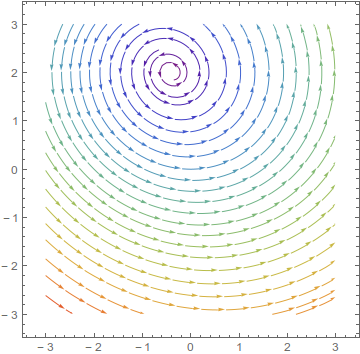
\includegraphics[scale=0.3]{spz-2} & 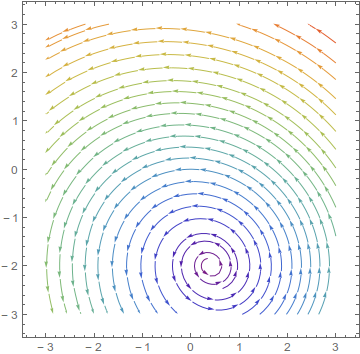
\includegraphics[scale=0.3]{spz2}\\
			$z=-2$ & $z=2$
		\end{tabular}
	\end{center}
	\pause
	\begin{itemize}
		\item Actually appears to be a spiral
	\end{itemize}
\end{frame}

\begin{frame}{Linearization}
	\begin{itemize}
		\item Can analyze the other fixed point
		\pause
	\end{itemize}
	\begin{gather*}
		\left|J\left(c,-\frac{c}{a},\frac{c}{a}\right) -\lambda I\right| =
		\frac{ ac - a\lambda - c\lambda + a^{2}\lambda^{2} -a\lambda^{3}}{a}.
	\end{gather*}
	\pause
	\begin{itemize}
		\item Solving with Mathematica yields bad values
		\pause
		\item Recall system was meant to be analyzed with small $a,b$
		\pause
		\item Let $a\to0.14$, $c\to8.8$
	\end{itemize}
	\pause
	\[
		\lambda =0.001-7.99i\pause\qquad \lambda=0.001+7.99i\pause\qquad\lambda=0.13
	\]
	\pause
	\begin{itemize}
		\item $\therefore$ fixed point is an unstable focus node
	\end{itemize}
\end{frame}

\begin{frame}{Chaos}
	\begin{center}
		
\includegraphics[scale=0.2]{bane}
	\end{center}
	\pause
	\begin{itemize}
		\item Mathematica demonstration
	\end{itemize}
\end{frame}

\begin{frame}{Chaos}
	\begin{itemize}
		\item Small changes in the system yield drastic changes in behavior
		\pause
		\item Periodicity changes to chaotic behavior
	\end{itemize}
	\pause
	\begin{center}
		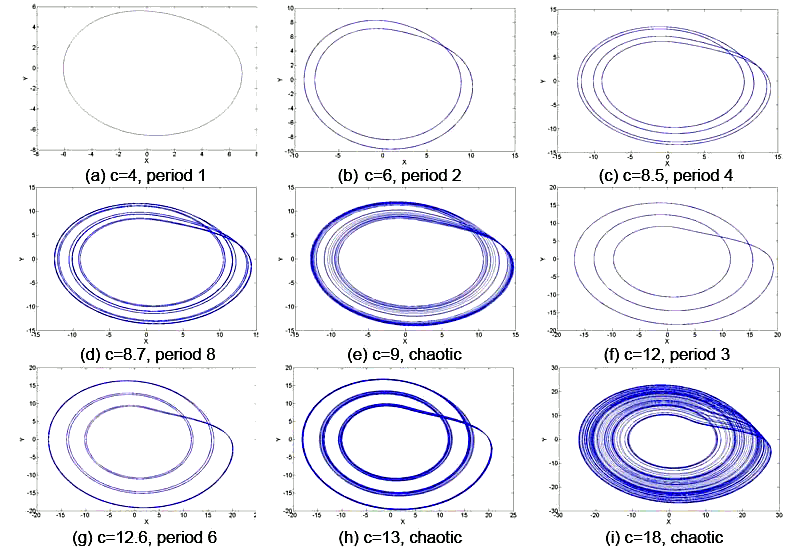
\includegraphics[scale=0.3]{varying_c}
	\end{center}
\end{frame}

%can talk about atrractiveness if need more time
\begin{frame}{References}
	\nocite{*}
	\bibliographystyle{alpha}
	\bibliography{mbib}
\end{frame}

\end{document}
